\documentclass[14pt,a4paper,report]{report}
\usepackage[a4paper, mag=1000, left=2.5cm, right=1cm, top=2cm, bottom=2cm, headsep=0.7cm, footskip=1cm]{geometry}
\usepackage[utf8]{inputenc}
\usepackage[english,russian]{babel}
\usepackage{indentfirst}
\usepackage[dvipsnames]{xcolor}
\usepackage[colorlinks]{hyperref}
\usepackage{listings} 
\usepackage{fancyhdr}
\usepackage{caption}
\usepackage{graphicx}
\hypersetup{
	colorlinks = true,
	linkcolor  = black
}

\usepackage{titlesec}
\titleformat{\chapter}
{\Large\bfseries} % format
{}                % label
{0pt}             % sep
{\huge}           % before-code


\DeclareCaptionFont{white}{\color{white}} 

% Listing description
\usepackage{listings} 
\DeclareCaptionFormat{listing}{\colorbox{gray}{\parbox{\textwidth}{#1#2#3}}}
\captionsetup[lstlisting]{format=listing,labelfont=white,textfont=white}
\lstset{ 
	% Listing settings
	inputencoding = utf8,			
	extendedchars = \true, 
	keepspaces = true, 			  	 % Поддержка кириллицы и пробелов в комментариях
	language = C,            	 	 % Язык программирования (для подсветки)
	basicstyle = \small\sffamily, 	 % Размер и начертание шрифта для подсветки кода
	numbers = left,               	 % Где поставить нумерацию строк (слева\справа)
	numberstyle = \tiny,          	 % Размер шрифта для номеров строк
	stepnumber = 1,               	 % Размер шага между двумя номерами строк
	numbersep = 5pt,              	 % Как далеко отстоят номера строк от подсвечиваемого кода
	backgroundcolor = \color{white}, % Цвет фона подсветки - используем \usepackage{color}
	showspaces = false,           	 % Показывать или нет пробелы специальными отступами
	showstringspaces = false,    	 % Показывать или нет пробелы в строках
	showtabs = false,           	 % Показывать или нет табуляцию в строках
	frame = single,              	 % Рисовать рамку вокруг кода
	tabsize = 2,                  	 % Размер табуляции по умолчанию равен 2 пробелам
	captionpos = t,             	 % Позиция заголовка вверху [t] или внизу [b] 
	breaklines = true,           	 % Автоматически переносить строки (да\нет)
	breakatwhitespace = false,   	 % Переносить строки только если есть пробел
	escapeinside = {\%*}{*)}      	 % Если нужно добавить комментарии в коде
}

\begin{document}

\def\contentsname{Содержание}

% Titlepage
\begin{titlepage}
	\begin{center}
		\textsc{Санкт-Петербургский Политехнический 
			Университет Петра Великого\\[5mm]
			Кафедра компьютерных систем и программных технологий}
		
		\vfill
		
		\textbf{Отчёт по лабораторной работе №1\\[3mm]
			Курс: «Интеллектуальные системы»\\[41mm]
		}
	\end{center}
	
	\hfill
	\begin{minipage}{.4\textwidth}
		Выполнил студент:\\[2mm] 
		Волкова М.Д.\\
		Группа: 13541/2\\[5mm]
		
		Проверил:\\[2mm] 
		Сазанов А.М.
	\end{minipage}
	\vfill
	\begin{center}
		Санкт-Петербург\\ \the\year\ г.
	\end{center}
\end{titlepage}

% Contents
\tableofcontents
\clearpage

\chapter{Лабораторная работа №1}

\section{Цель работы}

Научиться оформлять отчеты по лабораторным работам.

\section{Программа работы}

\begin{enumerate}
	\item Приведите развернутое определение следующих понятий: Интеллект, Ум, Разум, Мышление, Интуиция, Чувства, Инстинкт, Творчество. Что в этих понятиях общего и в чем различия? Что по вашему мнению отличает человеческое мышление от животного? Приведите
	примеры. Является ли биологический аспект (живое существо или машина) главным при принятии
	решения о разумности (интеллектуальности) объекта?
	
	\item Что такое интеллектуальная система? Какую систему можно назвать «по-настоящему»
	интеллектуальным? Приведите примеры «интеллектуальных» систем, и наоборот систем
	которые считаются «интеллектуальными» но по-вашему таковыми не являются.
	
	\item В чем отличия следующих понятий: события, факты, знания, данные?
	
	\item Приведите современную классификацию интеллектуальных систем и представлений знаний
	в этих системах.
	
	\item Перечислите и по возможности классифицируйте основные существующие системы принятия решения. Выявите общие черты и различия.
	
	\item Все ли знания могут быть формализованы? Можно ли ожидать решения задачи создания в
	полном смысле слова искусственного интеллекта? Обоснуйте свою точку зрения.
	
	\item Какие события, открытия, изобретения или гипотезы в области ИС наиболее перспективны по вашему мнению?
	
	\item Приведите пример ТОП-5 технологий, которые по Вашему вниманию уже сейчас активно
	меняют наш мир.
\end{enumerate}

\clearpage

\section{Ход работы}

\subsection{Задание 1}

\subsubsection{Приведите определение следующих понятий: Интеллект, Ум, Разум, Мышление, Интуиция, Чувства, Инстинкт, Творчество}

\emph{\textbf{Интеллект}} -- в общем смысле способность мыслить; в гносеологии – способность к опосредованному, абстрактному познанию, включающая в себя такие функции, как сравнение, абстрагирование, образование понятий, суждение, умозаключение; противостоит непосредственным видам познания – чувственному и интуитивному; в психологии – рациональное, подчиненное законам логики мышление; противостоит нерациональным сферам психики – эмоциям, воображению, воле и т.д. [1]

\emph{\textbf{Ум}} -- характерная способность мышления и понимания [2]

\emph{\textbf{Разум}} -- философская категория, выражающая высший тип мыслительной деятельности, противопоставляемый рассудку [3]

\emph{\textbf{Мышление}} -- высшая форма познавательной деятельности человека, социально обусловленный психический процесс опосредованного и обобщенного отражения действительности, процесс поисков и открытия существенно нового [4]

\emph{\textbf{Интуиция}} -- безотчётное неосознанное чувство, подсказывающее правильное поведение, понимание чего-либо, чутьё [5]

\emph{\textbf{Чувства}} -- средства восприятия организмом информации о внешней среде и об его (организма) физиологическом состоянии. Пяти чувствам (зрению, слуху, осязанию, обонянию и вкусу) соответствуют специализированные рецепторы, находящиеся на поверхности тела или вблизи от него. сенсорные (чувствительные) нейроны несут информацию от органов чувств к мозгу. Более того, рецепторы внутри тела улавливают внутренние физические и химические изменения [6] 


\emph{\textbf{Инстинкт}} -- поведение, обусловленное врожденными реакциями в отличие от поведения, обусловленного приобретенными навыками [7]


\emph{\textbf{Творчество}} -- деятельность человека, направленная на создание культурных или материальных ценностей [8]



\subsubsection{Что в этих понятиях общего и в чем различия?}

Все понятия тесно связаны друг с другом. Различая, на мой взгляд, между понятиями заключаются в уровне на котором они расположены. Так интуицией человек обладает с рождения и ее нельзя развить. Чувствами человек тоже обладает с рождения, но их можно совершенствовать. А разум – явление более высокое, чем ум и чувства. Ум человека в основном занят тем, что принимает приятное ему и отвергает неприятное. Разум также способен принимать и отвергать, но сосредоточен он на выборе благоприятного для человека и отбрасыванию опасного, неблагоприятного. Таким образом, их функции схожи, но разум обладает большей дальновидностью, стремясь определить пользу и вред.

\subsubsection{Что по вашему мнению отличает человеческое мышление от животного? Приведите примеры}

На этот вопрос ответить довольно трудно. По-моему мнению, человек, в отличае от животного, может мыслить в абстрактных понятиях, ему доступно воображение. Мышление же животных сводится к врожденным инстинктам.

\subsubsection{Является ли биологический аспект главным при принятии решения о интеллектуальности объекта?}

Нет. Если попробовать создать человеческий мозг, то сохранится вся его функциональность. Однако, в настоящее время это невозможно, ввиду энергозатрат.

\subsection{Задание 2}

\subsubsection{Что такое интеллектуальная система?}

\emph{\textbf{Интеллектуальная система}} -- это техническая или программная система, способная решать задачи, традиционно считающиеся творческими, принадлежащие конкретной предметной области, знания о которой хранятся в памяти такой системы. Структура интеллектуальной системы включает три основных блока — базу знаний, механизм вывода решений и интеллектуальный интерфейс [9] 

\subsubsection{Какую систему можно назвать «по-настоящему» интеллектуальной?}

Интеллектуальной системой можно назвать ту, которая способна принимать решения самостоятельно.

\subsubsection{Приведите примеры «интеллектуальных» систем, и наоборот систем, которые считаются «интеллектуальными», но по-вашему таковыми не являются.}

Системы распознования речи, переводчики, системы, которые переводят рукописный текст в электронный.

Некоторые виртуальные боты, которые используют шаблоны ответов, но при этом базируются на нейронных сетях, я считаю, не интеллектуальными системами (потому что их можно разложить на развлетленные алгоритмы).

\subsection{Задание 3}

\subsubsection{В чем отличия следующих понятий: события, факты, знания, данные?}

\emph{\textbf{Событие}} -- то, что имеет место, происходит, наступает в произвольной точке пространства-времени; значительное происшествие, явление или иная деятельность как факт общественной или личной жизни; множество исходов эксперимента [10]

\emph{\textbf{Факт}} -- называется утверждение, информационное сообщение и т. д., которые отражают действительность, являются правдивыми [11]

\emph{\textbf{Знание}} -- результат познавательной деятельности человека [12]

\emph{\textbf{Данные}} -- факты и характеризующие их числовые, количественные показатели: имена, даты событий, сведения об экономических процессах, местах действия [13]

\subsection{Задание 4}

\subsubsection{Приведите современную классификацию интеллектуальных систем и представлений знаний в этих системах}

\begin{figure}[h!]
	\centering
	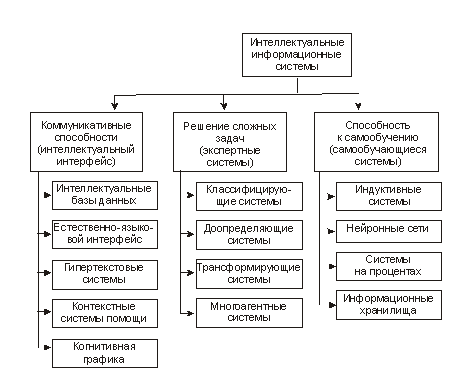
\includegraphics[scale = 1.40]{images/iis.png}
	\caption{Классификация ИИС [14]}
	\label{image:1}
\end{figure}	


\subsection{Задание 5}

\subsubsection{Перечислите и по возможности классифицируйте основные существующие системы принятия решения. Выявите общие черты и различия}

По взаимодействию с пользователем выделяют три вида СППР [15]:

\begin{itemize}
	\item пассивные помогают в процессе принятия решений, но не могут выдвинуть конкретного предложения;
	\item активные непосредственно участвуют в разработке правильного решения;
	\item кооперативные предполагают взаимодействие СППР с пользователем. Выдвинутое системой предложение пользователь может доработать, усовершенствовать, а затем отправить обратно в систему для проверки. После этого предложение вновь представляется пользователю, и так до тех пор, пока он не одобрит решение.
\end{itemize}

По способу поддержки различают [15]:

\begin{itemize}
	\item модельно-ориентированные СППР, используют в работе доступ к статистическим, финансовым или иным моделям;
	\item СППР, основанные на коммуникациях, поддерживают работу двух и более пользователей, занимающихся общей задачей;
	\item СППР, ориентированные на данные, имеют доступ к временным рядам организации. Они используют в работе не только внутренние, но и внешние данные;
	\item СППР, ориентированные на документы, манипулируют неструктурированной информацией, заключенной в различных электронных форматах;
	\item СППР, ориентированные на знания, предоставляют специализированные решения проблем, основанные на фактах.
\end{itemize}	
	
По сфере использования выделяют [15]:

\begin{itemize}
	\item общесистемные;
	\item настольные СППР.
\end{itemize}

Общесистемные работают с большими СХД и применяются многими пользователями. Настольные являются небольшими системами и подходят для управления с персонального компьютера одного пользователя [15]

\subsection{Задание 6}

\subsubsection{Все ли знания могут быть формализованы?}

Нет. Например, умение ездить на велосипеде (держать равновесие).

\subsubsection{Можно ли ожидать решения задачи создания в полном смысле слова искусственного интеллекта? Обоснуйте свою точку зрения.}

В дальнейшей перспективе, может быть, и возмоно. Все зависит от успехов в области изучения человеческого мозга, а и вычислительных способностей.

\subsection{Задание 7}

\subsubsection{Какие события, открытия, изобретения или гипотезы в области ИС наиболее перспективны по вашему мнению?}

С ростом вычислительных способностей и огромного количества данных в открытым доступе, наиболее перспективным, по-моему мнению, является глубокое обучение.

\subsection{Задание 8}

\subsubsection{Приведите пример ТОП-5 технологий, которые по Вашему вниманию уже сейчас активно меняют наш мир.}

\begin{itemize}
	\item текстовое описание по картинке
	\item обработка естественного языка
	\item анализ временных рядов
	\item прогнозирование временных рядов
	\item компьютерное зрение
\end{itemize}

\section{Вывод}

В данной работе были рассмотрены понятия, события, перспективы, технологии, которые относятся к данной предметной области. А также, основные проблемы создания ИИ.

\clearpage

\section{Список литературы}

% [16] https://geektimes.ru/post/280912/

% \linebreak

\begin{flushleft}

[1] Большая совестская энциклопедия [Электронный ресурс]. — URL: https://gufo.me/dict/bse/Интеллект

[2] Большая совестская энциклопедия  [Электронный ресурс]. — URL: https://gufo.me/dict/abbreviationstech/УМ

[3] Малый академический словарь [Электронный ресурс]. — URL: https://gufo.me/dict/mas/разум


[4] Малый академический словарь [Электронный ресурс]. — URL: https://gufo.me/dict/mas/мышление

[5] Толковый словарь Кузнецова [Электронный ресурс]. — URL: https://gufo.me/dict/kuznetsov/интуиция

[6] Научно-технический словарь [Электронный ресурс]. — URL: https://gufo.me/dict/scientific/ЧУВСТВА


[7] Научно-технический словарь [Электронный ресурс]. — URL: https://gufo.me/dict/scientific/ИНСТИНКТ

[8] Малый академический словарь [Электронный ресурс]. — URL: https://gufo.me/dict/mas/творчество

[9] Интеллектуальные системы [Электронный ресурс]. — URL: https://www.intuit.ru/studies/courses/46/46/lecture/1368


[11] Событие - Психологос [Электронный ресурс]. — URL: http://www.psychologos.ru/articles/view/sobytie

[12] Толковый словарь Дмитрива [Электронный ресурс]. — URL: http://dic.academic.ru/dic.nsf/dmitriev/5687

[13] Знание - определение [Электронный ресурс]. — URL: psihotesti.ru/gloss/tag/znanie/

[14] Данные [Электронный ресурс]. — URL: https://tochka.com/info/glossary/ДАННЫЕ

[15] ВГУЭС. Информационные технологии в экономике [Электронный ресурс]. — URL: https://abc.vvsu.ru/books/upinformtehnolvekon/page0017.asp

\end{flushleft}
	


\end{document}